%\section{Results -- $RQ1$}
%\label{sec:results-RQ1}
%Recall that in Section~\ref{sec:intro} we stated 
%This section presents and analyses the results of the survey.
In some cases we quote the survey respondents using [R$N$] to refer to a quote coming from respondent numbered $N$.
%\ad{Do we really need to make this distinction in the notation? I mean: I only see one example of R2-X, and if it matters, we can still make it explicit in the text. If we decide to ignore the difference between attached and detached variants, I even suggest to remove it from the Method section.}
%Codes resulting from coding open-ended answers are \dashuline{underlined}. Open ended responses from the participants are presented in \emph{italics}. Where applicable, we integrate and compare our findings with related research findings.

\begin{figure*}[ht]
\centering
\vspace{-.3cm}
    \hfill
        \subfigure[Was the motivation for creating the variant an individual decision or a community decision?]{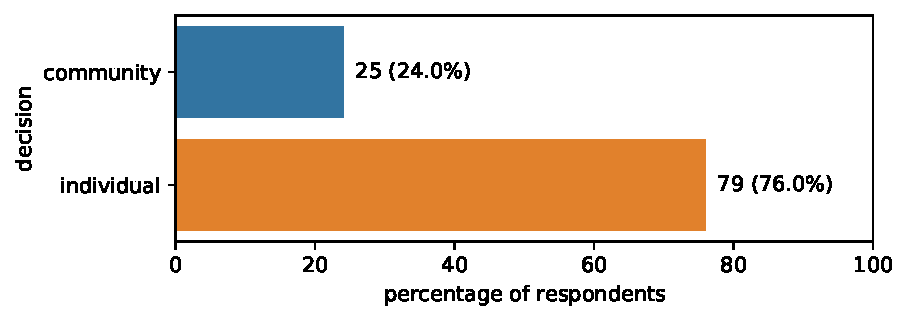
\includegraphics[width=1\columnwidth]{pdfs/decision.pdf}
        \label{fig:decision}}
    \hfill
    \subfigure[What was the motivation of creating the variant of the mainline project?]{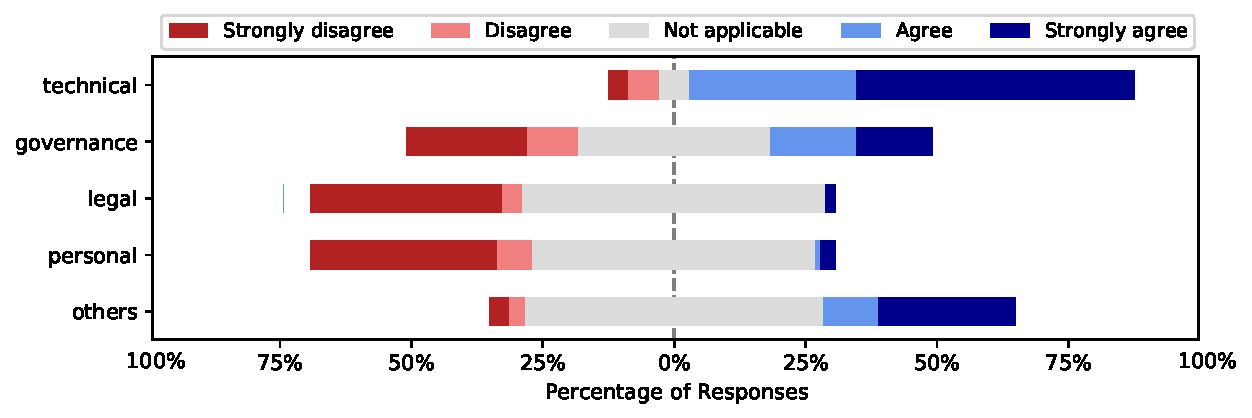
\includegraphics[width=1\columnwidth]{pdfs/likert_motivations_1.pdf}
    \label{fig:motivations}}
    \hfill
    \caption{\RQTwo}
     \label{fig:decision_motivations}
     \vspace{-.3cm}
\end{figure*}

\section{Results -- $RQ1$}
\label{sec:results-RQ1}
Recall that in Section~\ref{sec:intro} we stated \textbf{\RQOne} The goal of this RQ was to investigate whether the motivations for creating variant forks identified before the advent of social coding platforms still hold or whether new factors have come into play since then. To do so, we asked the survey participants the following questions:

\begin{itemize}
\item \rqOneOne
\item \rqOneTwo
\item \rqOneThree
\end{itemize}

$SQ1_{c}$ had open-ended answer. We coded the respondent's answers into themes to and categorised common responses.
When quoting the survey respondents, we refer to them using [R$N$] notation, where $N$ is the respondent's ID.
The respondents answers that include the selection on the multiple choice answers as well as the themes resulting from coding open-ended answers are \dashuline{underlined}. The
open-ended responses from the participants are presented in \emph{italics}. 
Where applicable, we integrate and compare our findings with related research findings.

% We now presents and analyses the results of the survey.
% In some cases we quote the survey respondents using [R$N$] to refer to a quote coming from respondent numbered $N$.

For $SQ1_{a}$ we presented a multiple choice question, $SQ1_{b}$ we presented Likert scale answer options and $SQ1_{c}$ was an open ended optional question.
 Fig.~\ref{fig:decision_motivations} presents the results of the responses for $SQ1_{a}$ and $SQ1_{b}$. Fig.~\ref{fig:decision} shows that the majority of the participants selected the option \dashuline{individual}. Fig.~\ref{fig:motivations} shows that the majority ranked highly the motivation \dashuline{technical}. We also see quite a number of highly ranked motivations of \dashuline{governance} and \dashuline{others}. In Fig.~\ref{fig:sankey_motivation} we can also see the association between the $SQ1_{a}$ and $SQ1_{b}$ on the axes of \dashuline{decision} and \dashuline{motivation}. We can see that the majority of respondents selected \dashuline{individual} and selected \dashuline{technical}.

% Like we presented in Section~\ref{sec:protocal}, th
% is question had Likert scale answer options we identified in the literature. 2) \emph{Was the motivation for creating the variant an individual decision or a community decision?} This survey question had two multiple choice answers of: \emph{individual} or \emph{community} decision.

While previous studies have investigated the motivations for creating variants, no study has investigated the details of those motivations ($SQ1_{c}$) .
To identify these details, we asked two additional optional open-ended questions to allow the respondents provide us with details on their choice of Likert scale answer on the motivation. The two questions were: 
\begin{enumerate}
	\item \emph{Kindly provide details for your selected answer(s) on the motivation; }
	\item \emph{If there are any links that are documented relating to your choice of answers on motivation detail, kindly point us there}
\end{enumerate}

100 of the 105 respondents that attempted the survey gave us a the details of the motivation of creating the variant and 30 of the 100 provided us with extra links. Luckily, while we were coding the open-ended question (Cf. Section~\ref{sec:card_sorting}), we were able to identify the five missing details of the choice of motivation by looking at selected response as well as comparing contents of the mainline and variant repositories on \gh.

In Fig~\ref{fig:sankey_motivation} we present the details of the choice of motivation by the respondents. We discuss what the coded themes represent in the next paragraphs.
Fig~\ref{fig:sankey_motivation} also presents how the distribution of the responses across all the five questions relating to motivation and how they relate to each other. The thickness of the edge represents the frequency of respondents between two entities.
%The axis--\texttt{variant status} in Fig~\ref{fig:sankey_motivation} shows the variants that are attached to- or detached from the mainline repository as discussed in Section~\ref{sec:forks_and_participants}. 
We observe that
% in both the \dashuline{attached} and \dashuline{detached} variants 
the majority of respondents that answered the question \dashuline{\# original developers} selected \dashuline{none} implying that the majority of the variants were started by different developers.
Since the answers to $SQ1_{c}$ were presented on a Likert scale, participants were allowed to rank the appropriate motivation(s) that suits why they created the variant. While coding the motivations details, we identified respondents who ranked highly more than one motivation category and also provided a response in the open-ended question to support each of the highly ranked motivation category. In this scenario, each of the ranked highly motivation category would have a motivation detail for the same respondent. %\az{I added the following information and modified the text introducing each motivation (detail)}
At the end we found that 105 of the survey participants chose 145 motivation categories, i.e., 84 \dashuline{technical}, 34 \dashuline{governance}, 3 \dashuline{legal} and 24 chose \dashuline{others}. 

\begin{figure*}[ht]
\begin{center}
    \centering
    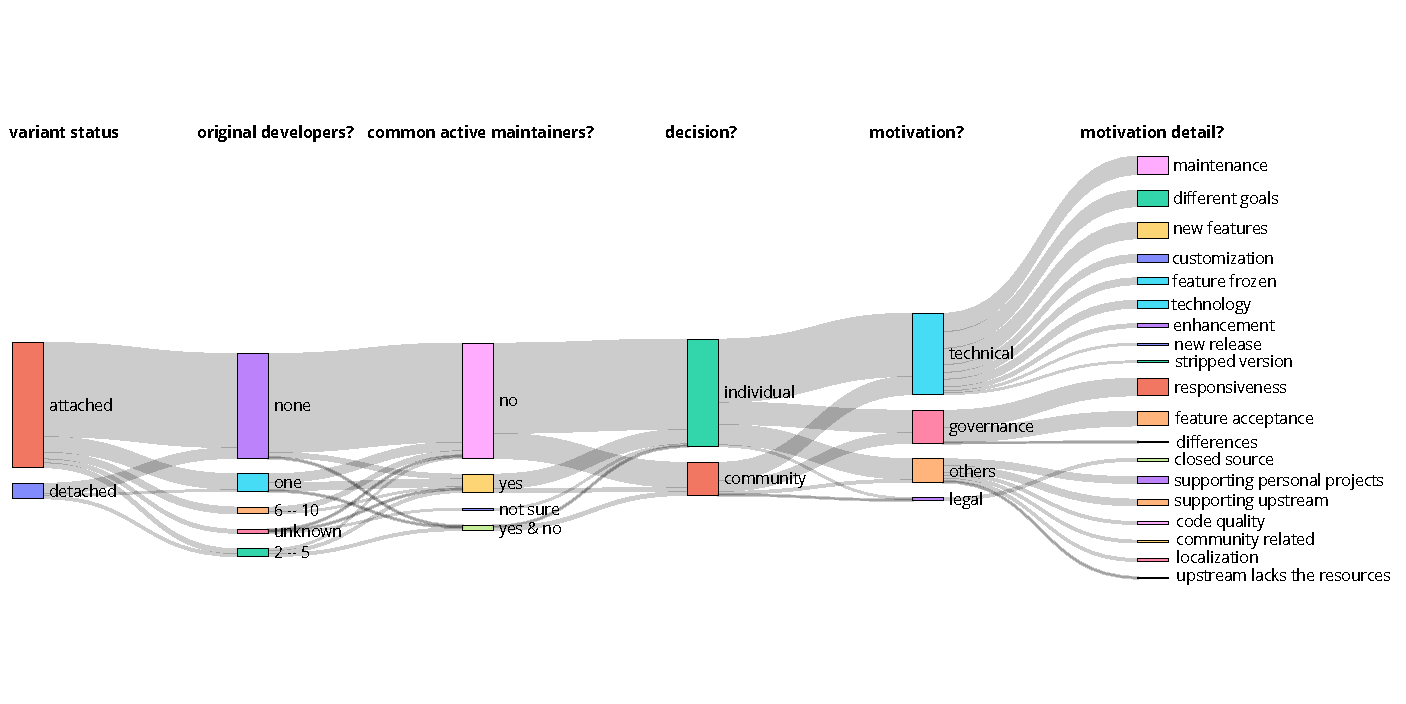
\includegraphics[width=\textwidth]{pdfs/sankey_motivations_2.pdf}
    \caption{Detailed motivations behind creating variant forks.
    }
    \label{fig:sankey_motivation}
\end{center}
\vspace{-.3cm}
\end{figure*}

\nd \textbf{Technical.} The motivation of \dashuline{technical} is connected to the most of the motivation details with the most prominent being \dashuline{maintenance}. 19 of the 84 survey participants who selected \dashuline{technical}, mentioned phrases related to \emph{performing bug/security fixes}.

\begin{itemize}[leftmargin=*]

%\item \emph{The fork was created because that is how you contribute changes back to a project on github, then the original maintainer of the project abandoned it making my fork the main actively developed one} [R38]. %This motivation detail can be related to the findings of Robles and Gonz{\'a}lez-Barahona~\cite{Gregorio:2012} who reported that one of the outcomes of forking is

\item ``\emph{The PR to merge the fork's new capabilities into the mainline code was too large, [...] %resulting in a long review time,
and my attempts to incorporate feedback into the PR [...] %(using force-pushes that disrupted the review process)
ended upsetting the primary maintainer who has been studiously ignoring the pull request for three years \frownie{}}'' [R59].
This respondent ranked highly both \dashuline{technical} and \dashuline{governance}. The respondent also provided a \gh link to their pull request to the mainline. Indeed, we found that the pull request was made in February 2018 and received 218 comments from both the mainline maintainer and the respondent discussing its details. On October 2021, the pull request is still open.

\item ``\emph{I forked the original project in order to fix a bug. However, the way the original was architected made this very challenging, so I ended up rewriting it instead of submitting a patch to the original}'' [R79].

\item ``\emph{The original project did not take WCAG accessibility guidelines into account. We first tried to make improvements on it, but they were broken soon after. So we finally decided to fork the project with the explicit aim to focus on accessibility}'' [R88]. A \gh issue link provided by the respondent showed that the question ``\textit{Did this start as an experiment or an intentional hard fork?}" was explicitly asked to the variant maintainers. The latter responded by mentioning that at first their intention was to improve the mainline and not maintain a different project, but later, some of their merged fixes were removed from the mainline. This led them continue maintaining their fork in a different way.
%\ad{That one seems more a ``different goal''.}\jb{I agree}\az{I am not sure if it different goals. Check my text above and https://github.com/KIProtect/klaro/pull/39}

\end{itemize}

\nd The next prominent \dashuline{technical} motivation detail was \dashuline{different goals}. 17 of the participants who selected \dashuline{technical}, mentioned phrases related to \emph{variants present different goals\,/\,content\,/\,communities\,/\,directions}.

\begin{itemize}[leftmargin=*]
\item ``\emph{[We] %Difference in content -
list websites that accept Bitcoin Cash cryptocurrency, as opposed to the mainline that lists websites with 2 factor authentication}'' [R1].
\item ``\emph{The original goal of the mainline is completely different from the fork variant. % While the projects are related in the sense that they share a similar code base, they are very different pieces of software
}'' [R4].
%\item ``\emph{This is a cryptocurrency, which introduced a completely different monetary policy, and consensus, while keeping many of the original features of the mainline. It is worth noting that [...] %, for the same principle, the mainline itself is a variant of another project% (bitcoin/bitcoin)}'' [R70].\az{we gave enough examples here)}
\item  ``\emph{We wanted to take the project in a different direction}'' [R100].
\end{itemize}

\nd The next prominent \dashuline{technical} motivation detail was \dashuline{new features}.
17 of the participants who selected \dashuline{technical}, mentioned phrases related to \emph{introduction of new features not in the mainline}.

\begin{itemize}[leftmargin=*]
\item ``\emph{[...] to add support for a feature I knew would not get merged into the main project}'' [R53].
\item ``\emph{Mainline developer only does bugfixes and eventual underlying runtime/SDK upgrades to stay current. He did not add new features due to lack of interest \ldots}'' [R67]
%\ad{This one better fits in ``feature frozen''}
%\jb{}
\item ``\emph{Our variant introduces new experimental functionality that is not yet ready for use in the mainline}'' [R80].
\end{itemize}

\nd The next prominent \dashuline{technical} motivation detail was \dashuline{customization}.
8 of the participants who selected \dashuline{technical}, mentioned phrases related to \emph{variant customizes the mainline features}.

\begin{itemize}[leftmargin=*]
\item ``\emph{The ``bones'' were good, but I wanted to add some aesthetics [...] %. Given the original prided itself on minimalism, it didn't feel right to contribute it into mainline.
so, I forked it to make it pretty and my own}'' [R10].
%\ad{Check the above quote. I removed an interesting part (``it didn't feel right to contribute it into mainline''). If you decide to keep it, then I suggest to move this quote to the ``different goals'' category.}
\item ``\emph{The new version is a vectorized, accelerated version of the original.%, but used some common code. It's not so much a fork as ``inspired by'', but we wanted to give due credit
}'' [R37].
\item ``\emph{[We] added some syntactic sugar and some improvements by itself \ldots}'' [R42].
%\ad{This last one would better fit in ``no longer maintained''.}
\end{itemize}

\nd The next prominent \dashuline{technical} motivation detail was \dashuline{unmaintained feature}.
8 of the participants who selected \dashuline{technical}, mentioned phrases related to \emph{one of the mainline feature used by the variant is no longer maintained}.
%\ad{I don't get the link between ``feature frozen'' and ``feature no longer maintained''. You can freeze a feature while maintaining it (e.g. by providing patches or improvements to it). I suggest to rephrase it to ``unmaintained feature''.}

\begin{itemize}[leftmargin=*]
\item ``\emph{The `shiny' component of mainline was declared to be no longer maintained around the time I created our fork. [\ldots] I did not like many of the architectural decisions of the original project, I opted to create a fork instead of volunteer to maintain the original.}'' [R65]. The respondent provided an extra link. An issue about `shiny' component was opened up in Jul 2015 and closed in Jul 2017. The issue contained 93 comments from 35 participants. When closing the issue the maintained stated that ``\textit{[...] If somebody or bodies from the community wants to fork the source code and run with it, they have my blessing [...]})''. The variant was created on Aug 2017.
%\ad{This one fits in ``new technology''.}
\item ``\emph{The mainline project had made a radical shift from providing one set of features %(pip-review + pip-dump)
to a different, disjoint set of features. % (pip-compile + pip-sync).
The maintainer had thought about it very well, but some users (including myself) had built their workflows around one of the old features. For this reason, I lifted that particular feature into a separate project that was also published under a different name to the package index.%For these historical reasons, the mainline and the variant are not really alternatives to each other; rather, they are complementary
}'' [R23]. The respondent also provided us a link, \gh \texttt{issue}, discussing the details. The \texttt{issue} was opened by the variant maintainer on July 2015 and was eventually closed on April 2018. The \texttt{issue} had 33 comments involving 17 participants. %\jb{need to link with other qns}.
%\ad{@John: I like this kind of ``anecdotal evidences'', but I'm missing how it contributes to the point. Also, there should be something wrong about the dates, since it means the issue was closed before its opening.}

\item ``\textit{Mainline dropped support for a small subset of the code and asked for community support to create a fork to support that subset}'' [R66].
%\ad{If a set of features is dropped, doesn't that mean the projects went into different directions? It's not only ``we do no want to maintain this feature'' but rather ``we removed it, if you need it, do your own project''. If I'm right, this means it better fits in the ``different goals'' or in ``new features'' category.}
\end{itemize}

\nd The next prominent \dashuline{technical} motivation detail was \dashuline{technology}.
7 of the participants who selected \dashuline{technical}, mentioned phrases related to \emph{variant created to depend on a different technology}.

\begin{itemize}[leftmargin=*]
\item ``\emph{Added support for Open Street Maps as an available map provider [\ldots] mainline was not willing to accept this kind of contribution.}'' [R8]. This was also ranked as a \dashuline{governance}. 
\item ``\emph{The mainline wasn't updated to use .NET Core which I was using in my project, so I updated it}'' [R29].
\item ``\emph{[...] to keep the source code compatible with the language/compiler version that we use (Swift / Xcode). [...] %Sometimes new versions of Swift break source compatibility, if we update (or not update when there is a new one) the compiler but
if the maintainer of the mainline is supporting a different one, then we could not compile our dependency anymore}'' [R54].
\end{itemize}

\nd \textbf{Governance}. The motivation of \dashuline{governance} is connected to the second most motivation details mentions, with the most prominent being \dashuline{responsiveness}. 18 of the 34 survey participants who selected \dashuline{governance}, mentioned phrases related to \emph{mainline was unresponsive to pull requests or issues for a long time}. Most of the respondents that ranked highly \dashuline{governance} as the motivation, also ranked highly other options of motivations. Only 4 of the 34 ranked only \dashuline{governance}.

%\ad{Very first quote seems to belong to this category}

\begin{itemize}[leftmargin=*]
\item ``\emph{[They] %The parent repo
had a series of commits that fixed functionality for newer PHP versions, but never made into a release. %The library was being used in an enterprise app using Composer/Packagist, which requires a new GitHub release to update the published library.
After waiting for more than a year for a release, a fork was done just to push a newer release into Composer/Packagist}'' [R21].

\item ``\emph{We submitted some bug fixes [...], %to the original repo
but didn't hear back from the maintainer for a while and needed to progress to meet our own goals so we forked. I followed up over email with the maintainer and he merged the patches about a month later, at which point we closed down and archived our fork and returned to using the mainline}'' [R15].
Merging back to the original corresponds to one the outcomes of variant forking reported by Robles and Gonz{\'a}lez-Barahona~\cite{Gregorio:2012}.
%\ad{That one suggests we wrongly identified the variant fork (since it has been active for only one month). I suggest to remove this quote.}

\item ``\emph{%\ldots created in order to submit PR into mainline. Its purpose has changed
[...] due to lack of response from mainline maintainer (more than months) and need of release. This lead to release of a new variant. [...] there is no intention to submit changes to mainline anymore (even when the first PR was merged into mainline after more than year)}'' [R56].
\end{itemize}

\nd The next prominent \dashuline{governance} motivation detail was \dashuline{feature acceptance}.
15 of the participants who selected \dashuline{governance}, mentioned phrases related to \emph{mainline hesitant to or not willing to accept feature}.

\begin{itemize}[leftmargin=*]
\item \emph{``TECHNICAL: Added support for Open Street Maps as an available map provider. GOVERNANCE: not exactly governance, but mainline was not willing to accept this kind of contribution"} [R8]. This was coded as \dashuline{technology} in \dashuline{technical}. The respondent also provided a \gh pull request link that contains extra information, that we examined. The pull request contained 45 conversations and 15 participants between June 2018 until March 2021 when it was closed.
%\ad{I suggest to remove this quote since it combines two distinct reasons, and we do not explain that a respondent could select more than one reason (and what we did when they did).}

\item ``\emph{Mainline was not ready to accept those changes in part because the maintainers were not responsive. Since that time all of the issues have been dealt with and my variant is no longer needed, though the infrastructure for creating a new release of the variant remains in place in the event that it might be needed in the future}'' [R44].

\item ``\emph{%Yes, there were attempts, but at then end
[...] even main repo maintainer was saying he is busy and please use your fork for thing X and Y. We don't know the exact reason why he stopped maintaining it and also did not allow us to maintain his repo}'' [R89]. In one of the multiple choice answers, the respondent indicated that the variant was created through a  \dashuline{community decision}.
The respondent also provided an extra link, in which we discovered that
%The respondent also provided extra links (two issues on the mainline) relating to the motivation of creating\,/\,maintaining the variant. 
% we found that the variant was created through a \dashuline{community decision}.
%In the issues the extra links, 
three contributors from the community were interested in a couple of new features that were missing in mainline, but the mainline maintainer seemed busy. At the end, two members of the community took over the fork maintenance and introduced the missing features and advertised the additions in the \textsf{readme.md} file of the fork as well as in the issue.

\end{itemize}


\nd \textbf{Others}. %The motivation of \dashuline{others} is connected to the second\az{I don't understand this. I will modify the text} most motivation details mentions, with the most prominent being \dashuline{supporting personal projects}. 
The most prominent motivation detail for \dashuline{others} motivation is  \dashuline{supporting personal projects}. 8 of the 24 survey participants who selected \dashuline{others}, mentioned phrases related to \emph{variant was created to support personal projects}.


\begin{itemize}[leftmargin=*]

\item ``\emph{%Fairly boring as it's a very small library.
[The] maintainer %of the ``mother'' repo
was not interested in a PR that added functionality needed by a project I'm developing. [It] was considerably easier to add the logic into the [new] library than bolt it on.%, so I forked the library
}'' [R18]. This was ranked as \dashuline{technical}, \dashuline{governance}, and \dashuline{others}. As we can see in the participant response we have phrases like ``\textit{adding logic}" (\dashuline{new features, technical}), ``\textit{was not interested in a PR}'' (\dashuline{feature acceptance, governance}), and ``\textit{functionality needed by a project I'm developing}'' (\dashuline{supporting personal projects, others}).

\item ``\emph{In Oct 2017 Twitch.TV has changed its API and these changes broke the mainline project. I used this project daily and needed to fix it ASAP. After quick fix I started to add my own features. [...] the mainline project has been fixed and refactored, but my other projects were already depending on my own fork}'' [R56].

\item ``\emph{%The main reason for forking (OTHER) is
[...] to make sure that no matter what happen to the mainline repository, we can maintain source access to this library, which is an essential dependency of our project. \ldots}'' [R54]. This response is inline with the findings of Nyman et al.~\cite{Linus:2012Perspectives} who reported that forking provides a mechanism for safeguarding against despotic decisions by the project lead, who is thus guided in their actions to consider the best interest of the community.

\end{itemize}

\nd The next prominent \dashuline{others} motivation detail was \dashuline{supporting mainline}.
7 of the participants who selected \dashuline{others}, mentioned phrases related to \emph{supporting mainline}.
%\ad{So far, my impression is that we already have many cases of mainline maintainers hesistant to or not willing to accept feature spread in the above categories, for some reasons. I don't really get what is different here.}

\begin{itemize}[leftmargin=*]
\item ``\emph{We have a fork that is the ``main fork'', which is eclipse, and the ``development fork'' is OpenTOSCA. In this case, our modling tool [\ldots] is only maintained as the fork [\ldots] we synchronize everything between both forks while the OpenTOSCA one is mainly used to develop new features, which are then pushed as PRs to the main fork}'' [R61].
%\ad{This seems like a social fork, mostly for PRs, but at a different level than the usual social fork.}

\item ``\emph{Preparation of mainline pull requests. mainline repo should not be spammed by WIP PRs by students. Supervisors do coaching and try to improve the quality by the initial mainline pull request. [\dots] Keeping the PR open on the fork, reduces the number of PRs}'' [R73].
%\ad{Same here.}

\item ``\emph{We needed a repository for tracking our ideas to keep the number of issues of the main repository low}'' [R83]. An extra link was provided, in which we found that the mainline and variant are owned by the same developer: ``\emph{this repository is used by [X] to make his ideas transparent. He collects the issues here to avoid flooding the ``official'' issue tracker. - Refined issues will be migrated to the official issue tracker}".
%\ad{This last example confirms that this last category is not well defined. It's not about ``mainline hesistant to or not willing to accept feature'' but rather to prevent the mainline to be flooded by students' PRs, attempts, etc.}
\end{itemize}

\nd The next prominent \dashuline{others} motivation detail was \dashuline{code quality}.
3 of the participants who selected \dashuline{others}, mentioned phrases related to \emph{mainline low code quality}.

\begin{itemize}[leftmargin=*]
\item ``\emph{%The main reason I forked was code-quality.
The mainline [...] % library works, but
was clearly written by someone who isn't a professional software engineer.% Also: mainline was not properly packaged (and still isn't AFAIK).
}'' [R63].

\item ``\emph{%I forked the original project in order to fix a bug. However,
The way the original was architected made this very challenging, so I ended up rewriting it instead of submitting a patch to the original}'' [R79].
\end{itemize}


\nd \textbf{Legal}. The motivation of \dashuline{legal} is connected to the least number of motivation details mentions, with the most prominent being \dashuline{responsiveness}. It had only 3 of the 105 survey participants that indicated phrases related to \dashuline{closed source}. Below we present their corresponding responses.
%\ad{I see three items. Do we have 3 ``most interesting responses'', or 3 excerpts from 2 responses?}

\begin{itemize}[leftmargin=*]
\item ``\emph{[The] main reason is creating [an] open source and commercial product which has much more features% and we just collect open source components and use them. Red5 server is one of the component of the product
}'' [R7]. This motivation detail was also categorised as: \dashuline{(new features, technical)} and \dashuline{(supporting personal projects, others)}.

\item ``\emph{5 years ago the permissions model for GitHub and Travis is not what it is today. I wanted to use Travis for CI/CD but if I granted Travis access to my primary github account, it would have read access to all the github repos [...], which would expose private customer code. I forked the repo [but] the permissions model has evolved [and I] %I have a pending task to switch to github actions for CI/CD on the main repo, and to
deleted the fork}'' [R24].

\item ``\emph{The founders of the mainline had been absent from the project for several years, but came back and booted the maintainers off and
[...] shifted the project to a closed source. %There was an attempt to reconcile differences [...], but the these issues were resolved (at least from the point of view of the maintainers, in reality the founders just pretended to be fine with it and secretly plotted for the next year to remove the maintainers from the project and ban them from every community to minimize a potential fork when they announced their plans to change the license
}'' [R36]. %The decision to create the fork was initiated by the \dashuline{closed source}.
%Ahmed: I commented the text below because I don't see its added value.
The respondent provided a link with extra information showing that three of the maintainers that were booted from the original project and a fourth one from the community joined forces and are now maintaining the variant. The variant currently has over 739 stars, is used by 35 developers, has 101 pull requests and 195 issues.
\end{itemize}


\subsection{Discussion and Implications--$RQ1$}
In this study we were mainly interested in finding out the motivations for creating and maintaining variants especially those that actively being maintained in parallel with their mainline counterparts.
We have identified that the decision to create the variants is mostly initiated by individuals and less by community.
Our findings in this RQ confirm the findings in the literature.
% The survey participants revealed that they created variants for technical, governance, legal reasons that are reported in literature.
Our study also extends the findings in literature by providing fine-grained reasons for creating and maintaining variants relating to the previously reported reasons.
Furthermore, our study has also revealed other reasons not listed in literature that respondents categorised as \dashuline{others}, that include: 1) supporting the mainline, 2) variant supporting other personal projects, 3) localization purposes and 4) variants developers not trusting the code quality of the mainline.
The findings of this RQ will be very useful in follow-up studies in investigating the co-evolution of mainline and variants.

In Fig.~\ref{fig:sankey_motivation} we also present an overview of how the detailed motivations relate to who is involved in creating and maintaining the variants. We can see that the motivations majorly relate to developers outside (82\%) the core contributors of the mainlines. We also observe quite a significant (24\%) number of respondents indicating that the decision to create the variant was initiated by the community. We have also observed from the open-ended responses, that before the transition from social to variant fork, some variant maintainers engage with the mainline maintainers through discussions in issues and pull requests. This is inline with the findings of Zhou et al. who reported that many variant forks start as social forks~\cite{Zhou:2020}

Besides the motivations for creating and maintaining of variants, the respondents have reported some interesting software reuse practices by the variants, like those categorized in the themes of: \dashuline{different goals}, \dashuline{new features}, \dashuline{customization}, \dashuline{technology}, \dashuline{supporting personal projects}, \dashuline{supporting upstream}, \dashuline{localization}. A specific example of [R70] categorized in the \dashuline{different goals} theme, stated that in the cryptocurrency world, all applications inherit code from the mother project \texttt{bitcoin/bitcoin}. Downstream applications also monitor their immediate upstream and other in the hierarchy for important updates like bug and security fixes as well as other specific updates. These cryptocurrency applications can be considered as a \textit{software family}~\cite{businge:2018icsme,businge:emse:2021}), that are part of dedicated project ecosystem~\cite{tommens:2020}, continuously reuse code among themselves.
There are other dedicated software ecosystems that exist like, \textsf{Eclipse}, \textsf{Atom}, and \textsf{Emacs}, programming language ecosystems like:  \java, \cp, \cpp, \py, \go, \rb, operating system ecosystems like: \textsf{macOS}, \textsf{Linux}, \textsf{Windows}, and \textsf{iOS}~\cite{tommens:2020} can contain variants.
To this end, our study opens up different research directions that can be aimed at deeply investigating these different reuse practices in \textit{software family} and software variants in general. A deeper understanding of these reuse practices can aid the development of tools that can support more efficient software reuse.

\begin{framed}
\noindent
\emph{\textbf{Summary--RQ1}:
We have observed that many variant forks start as social forks. The decision to create\,/\,maintain the forks is either from community (contributing up to 24\%) or as individual (76\%). We have also observed that the majority (82\%) of the developers creating the forks are outside the maintainers of the mainlines. We have presented 18 variant creation\,/\,maintenance motivation details categorized in the motivations of \dashuline{technical} (accounting 58\% of the responses), \dashuline{governance} (24\%), \dashuline{others} (16\%) and \dashuline{legal} (2\%). The detailed motivations in the \dashuline{others} category are newly introduced in the social coding era. We have also discussed some interesting software reuse classifications among variants.
}
\end{framed}


\begin{figure*}[ht]
\centering
\vspace{-.3cm}
    \hfill
        \subfigure[$SQ2_{a}$. How many mainline developers involved in creation of variant?]{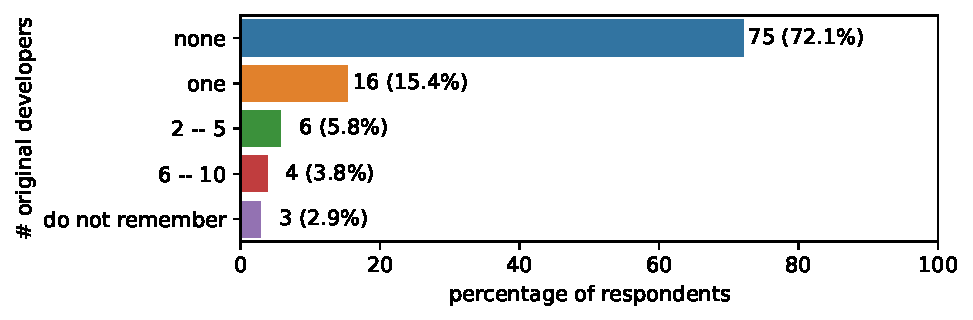
\includegraphics[width=1\columnwidth]{pdfs/original_developers.pdf}
        \label{fig:original}}
    \hfill
    \subfigure[$SQ2_{b}$. How many common active maintainers are there between mainline and variant?]{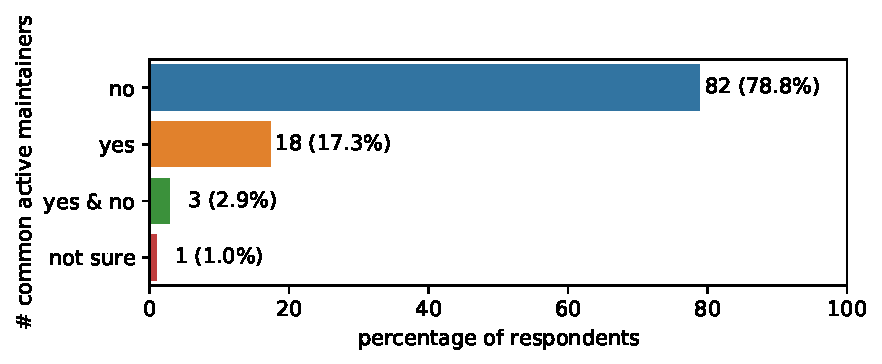
\includegraphics[width=1\columnwidth]{pdfs/common_maintainers.pdf}
    \label{fig:common}}
    \hfill
    \caption{Who are the developers involved in creating and maintaining variants of a mainline project?}
     \label{fig:original_common}
     \vspace{-.3cm}
\end{figure*}



\section{Results -- $RQ2$}
\label{sec:results-RQ2}
Recall that in Section~\ref{sec:intro} we stated \textbf{\RQTwo} The goal of this RQ was
to identify the impediments for co-evolution between the mainline and variant projects.
This RQ lead to two specific survey questions, reflecting the (\textit{who?}) and the (\textit{how}?), respectively. The \textit{who?} aimed at identifying the developers involved in maintaining these variants. The \textit{how?} aimed to understand how variant  projects actually evolve  w.r.t. the  mainline.

For the \textit{who} question, we asked the survey participants the following questions:

\begin{itemize}
\item  \rqTwoOne
\item \rqTwoTwo
\end{itemize}


Like in Section~\ref{sec:results-RQ1}, in this section we refer to the responses using the \dashuline{underlined}, \emph{italics} and [R$N$].
For both $SQ2_{a}$ and $SQ2_{b}$ we provided multiple choice answers to the questions. We present the results of $SQ2_{a}$ and $SQ2_{b}$ in Fig.~\ref{fig:original_common}. Looking at both Fig.~\ref{fig:original} and Fig.~\ref{fig:common} for both question respectively, we can see that the majority of the participants chose the options of \dashuline{none} (none of the creators of the variant were part of the mainline) and \dashuline{no} (they do not have common active maintainers).
This implies that the most of developers that are involved in the creation and maintenance of the variants are outside the core maintainers of the original project where the variant was forked.
The difference in the numbers of participants who selected  \dashuline{none} for $SQ2_{a}$ and \dashuline{no} for $SQ2_{b}$ can be visualized in Fig.~\ref{fig:sankey_motivation}.
When we look at how responses of $SQ2_{a}$--\dashuline{original developers?} and $SQ2_{b}$--\dashuline{common active maintainers?} are associated, we can see that the majority of the respondents that selected the option \dashuline{none} in $SQ2_{b}$ went ahead to select the option \dashuline{no} in $SQ2_{a}$. We can also see other associations between all responses of $SQ2_{a}$ and $SQ2_{a}$.
For example, in $SQ2_{a}$, the participant [R36] who selected the answer option \dashuline{6 -- 10} developers from the mainline were involved in creation of the variant, also selected the option \dashuline{yes \emph{\&} no}--\emph{``They used to have common maintainers in the early stages of the variant, but now the projects have technically diverged away from each other, there are no more common maintainers"} in $SQ2_{b}$.
We also observed that respondents [R51] and [R57] who selected the option \dashuline{6 -- 10} and \dashuline{2 -- 5}, respectively, for $SQ2_{a}$ also selected the option \dashuline{no} for $SQ2_{b}$. This implies that there were at least two maintainers involved in the creation of the fork, but none of those maintainers is currently contributing to both repositories.



The results of $SQ2_{a}$ and $SQ2_{b}$, answers to our question on \textit{who is creating and maintaining these variants?} Our observation is that the variants are created and maintained by developers different from those in the mainline counterparts. This observation conquers with the findings of an earlier study by Businge et al.~\cite{businge:emse:2021}.

%As opposed to our exploratory study surveying maintainers of variants, the study of Businge et al.~\cite{businge:emse:2021} was a large scale empirical study on mainline--variant pairs from three software ecosystems. They reported that over 82\% of the 10,979 mainline--variant are owned by different developers. In our study we have also found 82\% of variants are maintained by developers different from those in the mainline.

For the \textit{how} question, that aimed understanding how the projects co-evolve, we asked the survey participants the following questions:
\begin{itemize}
\item \rqTwoThree
\item   \rqTwoFour
\end{itemize}


\begin{figure}[ht]
\begin{center}
    \centering
    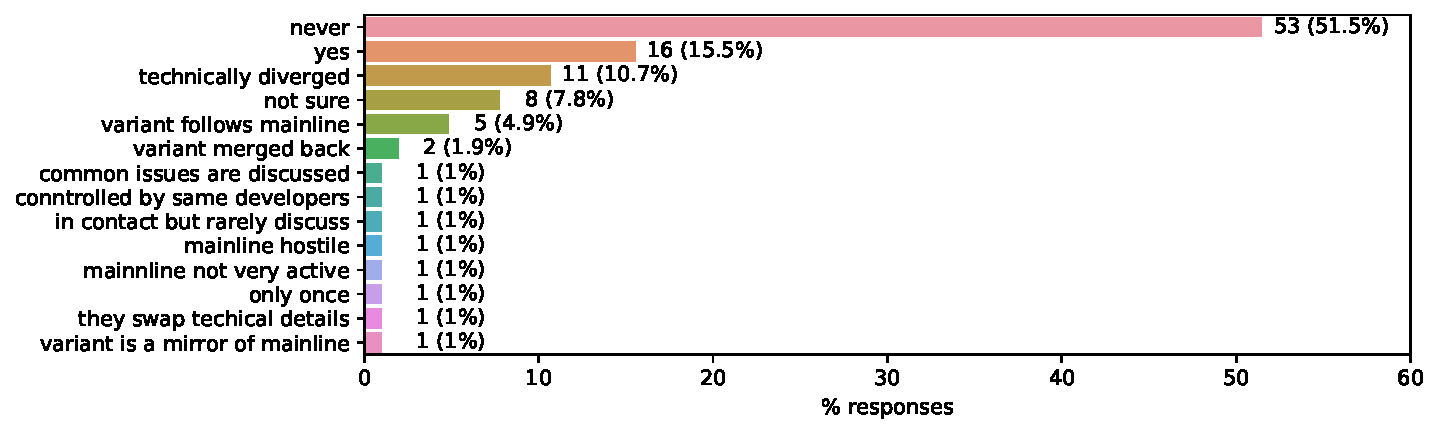
\includegraphics[width=\columnwidth]{pdfs/discussions_rq3_colored.pdf}
    \caption{$SQ2_{c}$ Do the variant forks and the mainline still discuss the main directions of the project?}
    \label{fig:discussions}
\end{center}
\vspace{-.3cm}
\end{figure}

\nd For $SQ2_{c}$ we presented four multiple choice answer options. From Fig.~\ref{fig:discussions}, the four answer options we provided for $SQ2_{c}$ are those with the highest number of responses. We also provided an option of an open-ended answer for participants who felt that their choice is not among the options. The open-ended answers were coded into themes (in Fig.~\ref{fig:discussions} the coded themes are \dashuline{variant follows mainline}\ra to \dashuline{variant is a mirror of the mainline}).
The results in Fig.~\ref{fig:discussions} show that more than 51\% of the responses chose the option of \dashuline{never}--\textit{no, there has never been any discussion since the creation of the variant}. In addition to the participants who selected \dashuline{never}, there are other variants that do not discuss the directions of the project, like \dashuline{mainline hostile} to variant,  \dashuline{mainline not very active},  \dashuline{in contact but rarely discuss}, \dashuline{only once}, and \dashuline{technically diverged}--``\emph{They used to discuss but not anymore since the projects have technically diverged from each other}''.

\begin{figure*}[t!]
\centering
\vspace{-.3cm}
    \hfill
        \subfigure[Code integration from mainline]{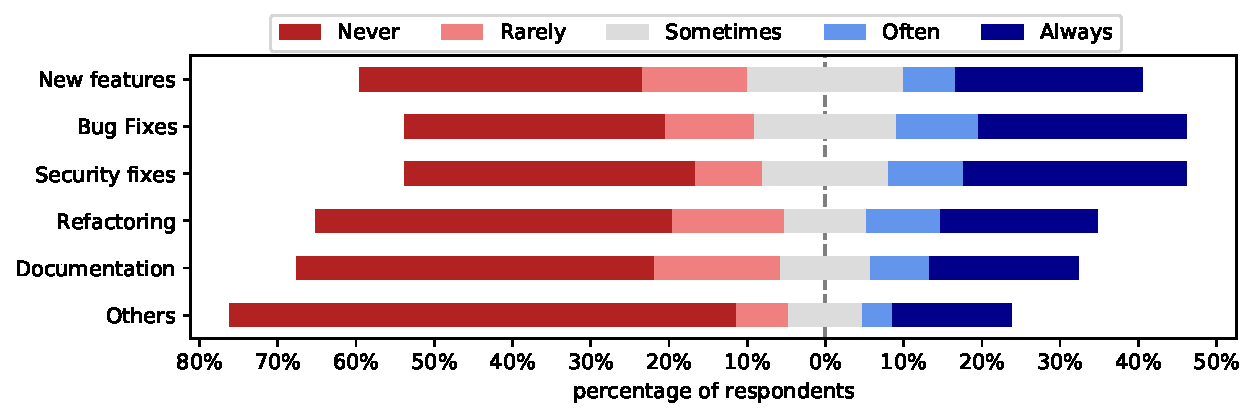
\includegraphics[width=1\columnwidth]{pdfs/likert_integration_from_mainline.pdf}
        \label{fig:from_mainline}}
    \hfill
    \subfigure[Code integration to mainline ]{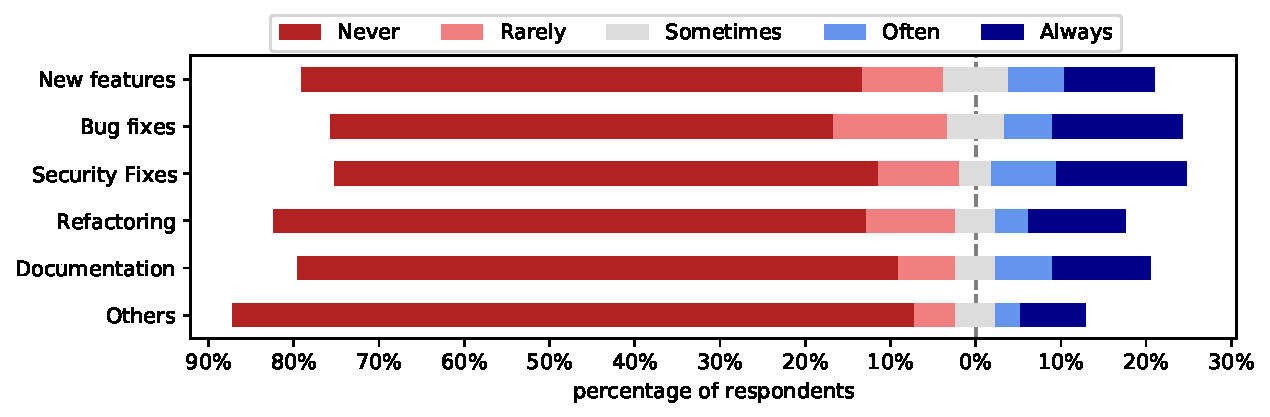
\includegraphics[width=1\columnwidth]{pdfs/likert_integration_to_mainline.pdf}
    \label{fig:to_mainline}}
    \hfill
    \subfigure[integration from mainline (coded themes)]{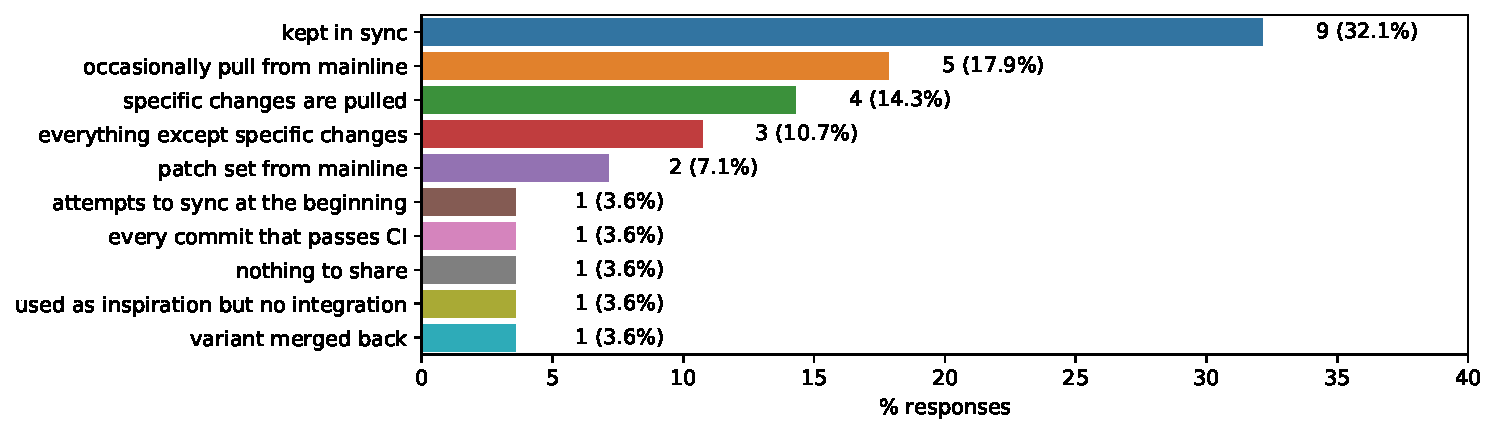
\includegraphics[width=1\columnwidth]{pdfs/changes_from_mainline.pdf}
        \label{fig:from_mainline-coded}}
    \hfill
    \subfigure[integration to mainline (coded themes) ]{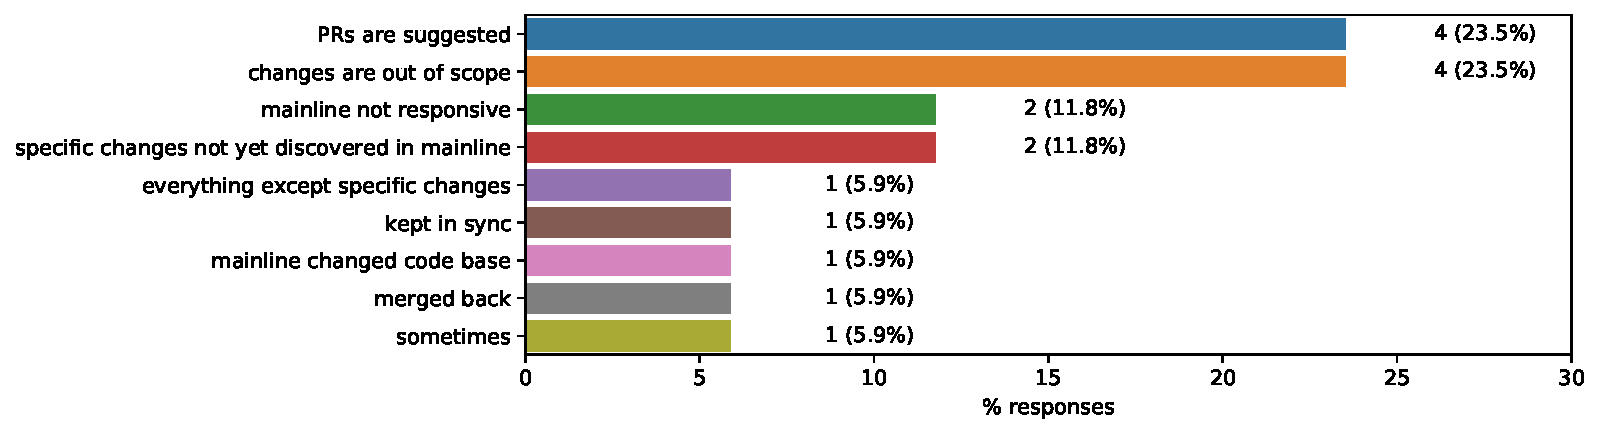
\includegraphics[width=1\columnwidth]{pdfs/changes_to_mainline.pdf}
    \label{fig:to_mainline-coded}}
    \hfill
    \caption{\RQTwo}
     \label{fig:interactions}
     \vspace{-.3cm}
\end{figure*}

An explanation for the high number of variants that do not discuss with the mainline the direction of the projects can be derived from the findings of $SQ2_{a}$ and $SQ2_{b}$, earlier, that the majority of the variants are created and maintained by developers outside the code developers of the mainline. Also most of the \emph{motivation details} in $RQ1$ could also explain the high numbers of \dashuline{never}. For example we have observed that the majority of the variants in the \emph{motivation details} category of \dashuline{different goals}, \dashuline{frozen features} in the mainline, those having issues with the mainline \dashuline{responsiveness}, those whose features will not be accepted by the mainline (\dashuline{feature acceptance}), selected  \dashuline{never} in $SQ2_{c}$. \textbf{To this end, we can conclude that the reasons for the majority of the variants not discussing the directions of the project with the mainlines could be attributed to the range of motivation details for creating the variant as well as the creators of the variants not being part of the core developers of the mainline.}
We found that 5 of the responses indicated phrases related to \dashuline{variant follows mainline}. For example respondent [R77] indicated that ``\emph{in the crypto world, the mainline inherits changes from BITCOIN, for example, security commits, and the variant merges those changes in. So the variant is very interested in every change in the Mainline. However, the variant must maintain the specific new features that we added separately, and the Mainline is not interested in helping the Variant do this.}''
We also observe two interesting cases where the variants merged back to the mainline. This is inline with the findings of Robles and Gonz{\'a}lez-Barahona~\cite{Gregorio:2012} who reported that one of the outcomes of forking is the fork merging back.



\nd In $SQ2_{d}$, we asked respondents two closed-ended questions: \textit{1) How often do the maintainers of the variant integrate the following types of changes from the mainline?} and\textit{ 2) How often do the maintainers of the variant integrate the following types of changes into the mainline?}
We provided Likert scale answers options for the two questions. We also asked the respondents optional follow-up questions with open-ended answers, for each of the two questions, to provide us with extra information.
%In Fig.~\ref{fig:interactions} we present the results of $RQ_{3.2}$.
In Fig.~\ref{fig:from_mainline} we present the results from the respondent answers on what they value most when integrating changes from the mainline. We can see that the highly scored changes are the \dashuline{bug fixes} and the \dashuline{security fixes}. In Fig.~\ref{fig:from_mainline} we can see that most of the respondents were leaning towards the negative side compared to the positive side of the plot.
This implies that most variants are not interested in integrating changes from the mainline.
In Fig.~\ref{fig:to_mainline} we see a similar trend observed in Fig.~\ref{fig:from_mainline}, however, the lean towards the negative side is much more pronounced in Fig.~\ref{fig:to_mainline}.
In Fig.~\ref{fig:from_mainline-coded} and Fig.~\ref{fig:to_mainline-coded} we present the coded themes of the extra information of the open-ended answer questions corresponding to the results in Fig.~\ref{fig:from_mainline} and Fig.~\ref{fig:to_mainline}, respectively. In Fig.~\ref{fig:from_mainline-coded} we present the results of 28 of the 105 participants who provided the extra information, while in Fig.~\ref{fig:to_mainline-coded} we present the results of 17 of the 105 participants.
This implies that most variants do not submit changes to the mainline.
In Fig.~\ref{fig:from_mainline-coded} we can see that the most prominent response was related to \dashuline{kept in sync} implying that the variants always keep in sync with the the changes made in the mainline. The next prominent response was related to \dashuline{occasionally pull from mainline} implying that variants from time to time pull changes made in the mainline. Some respondents mentioned phrases related to \dashuline{specific changes are pulled}; for example, [R63] indicated that ``\emph{It's mostly changes that make the library for specific iRobot Roomba models (new ones for example)}''. Other respondents mentioned phrases related to \dashuline{everything except specific changes}; for example, [R48] mentioned that \emph{All non-compiler specific changes are pulled}.
In Fig.~\ref{fig:to_mainline-coded} there were two most prominent answers: \dashuline{PRs are suggested}, for example, ``\textit{Made PRs with changes but those have just been ignored. They're still ``open'' with 0 comments from the mainline dev}'' [R67]. The other prominent answer is \dashuline{changes are out of scope}, for example, ``\emph{We use this as a dependency in another project [\ldots] which is often diverging from the language version of the mainline, so there is little reason for us to push this to mainline}'' [R54]. Another interesting theme is ``\emph{Only compiler non-specific that are discovered \ldots before they are discovered in upstream. [\ldots]}'' [R48].

\subsection{Discussion and Implications--$RQ2$}

The results of this study have revealed variants are created and maintained my developers outside the core developers of the mainlines.
We have also observed that there is limited interaction between the mainline and variant.
Although we find there is little code integration, the integration from mainline\ra variant is more than that from variant\ra mainline.
Our study confirms the findings of Businge et al.~\cite{businge:emse:2021} who carried out a large scale empirical study of code integration among mainline and variants from three ecosystem. Our study also extends the work of Businge et al.~\cite{businge:emse:2021} by providing some concrete reasons relating to little integration between the mainline and variants that include: 1) \textit{technical divergency}: where variants and mainlines are offering different goals, implementing different technologies, variant is maintaining a part of the mainline that is frozen. 2) \textit{Governance disputes}: mainlines are unresponsive to pull requests and issues from the variants and  mainlines not willing or hesitant to accept some features from the variants. One respondent also reported that mainline is actively very hostile to variant as a result of mainline changing licence to proprietary.
Another possible reason why the is little code integration is because most of the variants are created and maintained by developers outside the core developers of the mainline.
Furthermore, we have observed that a few mainline--variant pairs that integrate code between themselves are mostly interested in patch sets (security fixes and bug fixes).

Although maintenance and collaboration has on social coding platforms like \gh have improved through the tooling, especially distributed version
control systems like Git~\cite{Christian:MSR:2012} and transparency mechanisms on social coding platforms~\cite{Laura:2012:CSCW}, these tools are only ideal for social forks which aim to sync all the changes between repositories.
For example, code integration using pull requests and \texttt{git merge\,/\,rebase} may not be the best when integrating changes in between mainline and variant forks since they involve syncing upstream\,/\,downstream all the changes missing in the current branch.
In this study, we have observed that some variants maintainers are only interested in integrating commits with specific changes.
A suitable integration mechanism would be commit cherry picking since the developer can choose the exact commits they want to integrate.
However, \gh's current setup does not make it easy to identify commits to cherry-pick with out digging through the branch's history to identify relevant changes since the last code integration.
Additionally, even though the variants have diverged from their mainlines, we do believe that since they share common code, some of the common code may go through maintenance to perform some bug and security fixing. These mainline--variant repository pairs being maintained uncommon developers, chances are that these fixes could be missed or they could be fixed at different times by different developers and hence effort duplication.
Our findings can be very useful to code integration tool builders between mainline and variants to prioritise certain categories of mainline--variant pairs by targeting specific changes.
Ideally, a tooling would help identify possibly important fixes in commits and recommend these commits to mainline or variant developers to support a more efficient reuse.
Some promising studies in this direction have focused on providing the mainline with facilities to explore non-integrated changes in forks to find opportunities for reuse~\cite{Ren:2018}, cross-fork change migration~\cite{ray:2013:ASE,Ren:2019}. Also more experimental ideas about virtual product-line platforms for unified development of multiple variants of a project~\cite{Antkiewicz:icse:2014,Fischer:saner:2014,Montalvillo:spl:2015,rubin:icse:2013,Stefan:2016:icsme}.

\begin{framed}
\noindent
\emph{\textbf{Summary--RQ2}: We have observed that there is very little interaction between the mainline and variants during their co-evolution. The lack of interaction could be attributed to a number of reasons that include: (i) technical (i.e., diverging features), where variants and mainlines are offering different goals or implementing different technologies having nothing to share; (ii) governance (i.e., diverging interests), where mainlines are unresponsive to the requests from community and also uninterested in some features suggested by the community; (iii) legal (e.g., diverging licences), where the mainline variant has changed the licence and integration is no longer possible.
(iv) As a result of the divergence and since the majority of the variants are maintained by developers outside the core developers of the mainline, we report that its possible that some important updates (like patches) could be missed or are duplicated.
We also report interesting interactions that include: integration of only patches, integration of only specific changes, integration that exclude some specific changes and integration only changes that pass CI.
}
\end{framed}
